\section{Выполнение}

\subsection{Описание модели взаимодействия процессов}

Описание модели представлено в листинге \ref{lst:1}.

\begin{lstlisting}[label=lst:1,caption=Описание модели взаимодействия процессов.]
	short var1 = 3;
	short var2 = 2;
	short res1 = 0;

	byte busy = 0;

	proctype Thread1() {
		(busy == 0) -> busy++;
		assert(busy > 1);

		var1++;
		var2++;

		busy--;
	}

	proctype Thread2() {
		(busy == 0) -> busy++;
		assert(busy > 1);
		
		var1++;
		res1 = var1 + var2;

		busy--;
	}

	init {
		run Thread1();
		run Thread2();
	}
\end{lstlisting}

На рисунках \ref{img:1}-\ref{img:3} продемонстрированы логи SPIN, в которых видна гонка.

\begin{figure}[H]
	\centering
	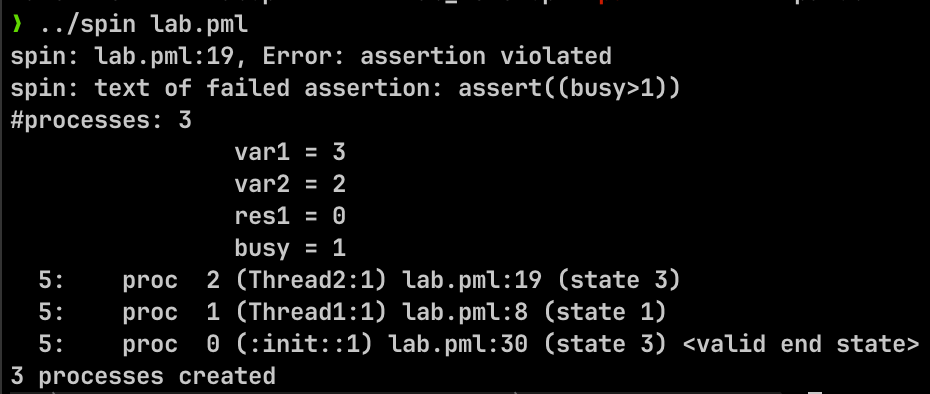
\includegraphics[width=\textwidth]{inc/1.png}
	\caption{ Логи SPIN, демонстрирующие гонку. }
	\label{img:1}
\end{figure}

\begin{figure}[H]
	\centering
	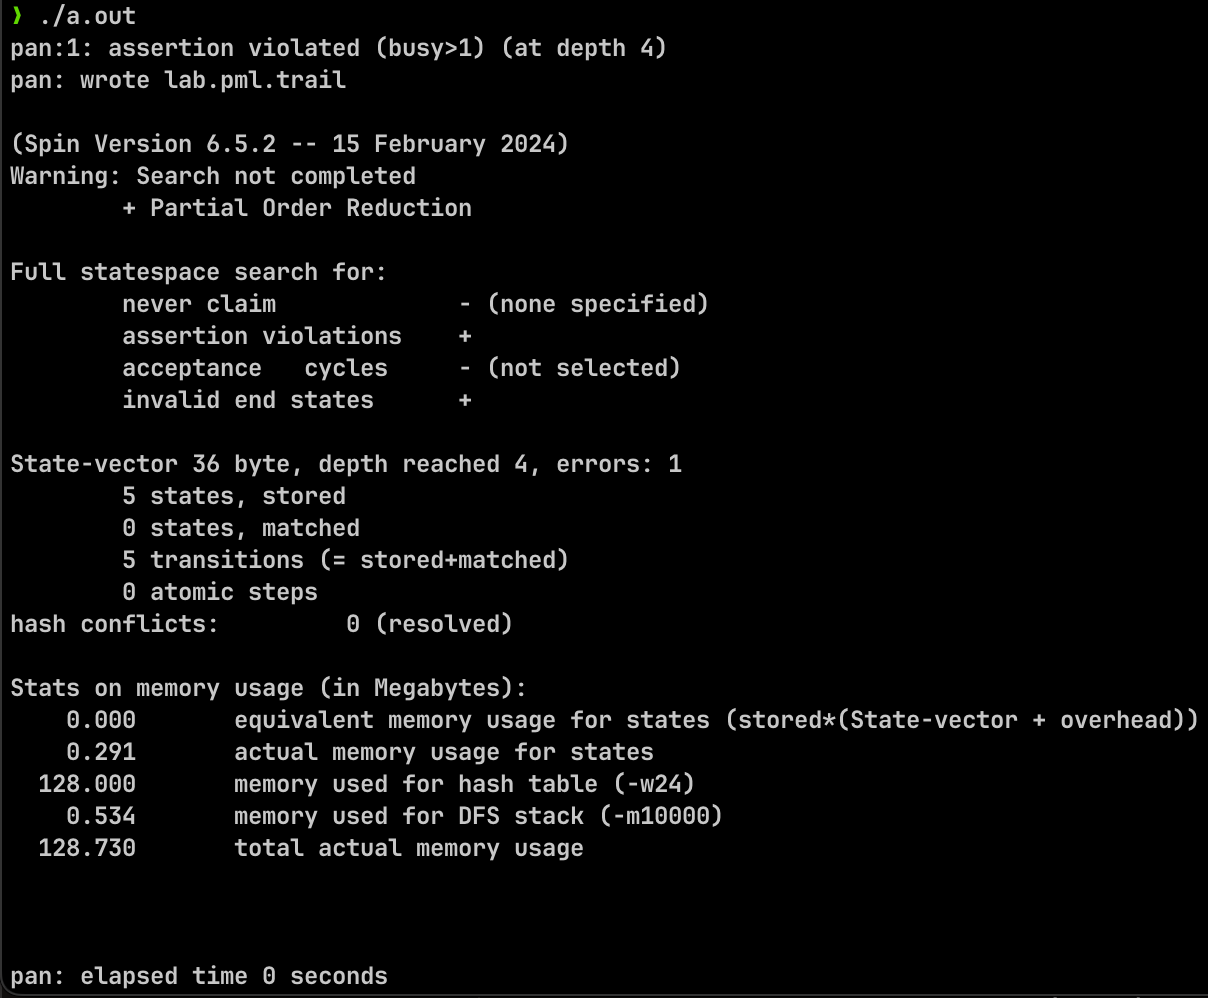
\includegraphics[width=\textwidth]{inc/2.png}
	\caption{ Логи SPIN, демонстрирующие гонку. }
	\label{img:2}
\end{figure}

\begin{figure}[H]
	\centering
	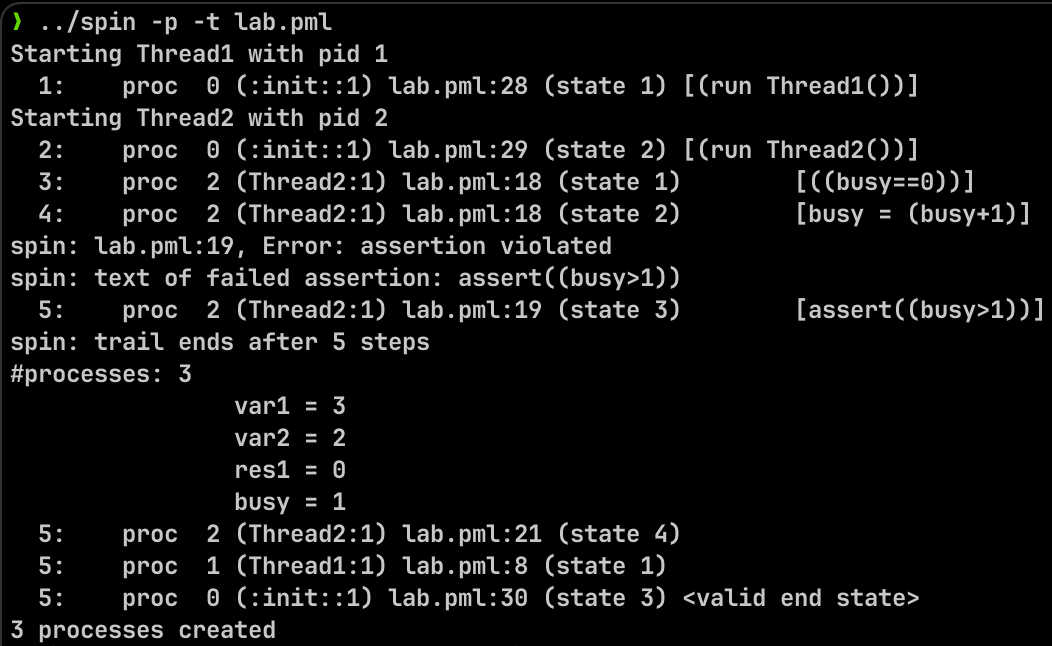
\includegraphics[width=\textwidth]{inc/3.png}
	\caption{ Логи SPIN, демонстрирующие гонку. }
	\label{img:3}
\end{figure}

Если не использовать ассерты, можно также отметить большую достигнутую глубину и количество результирующих состояний, на рисунке \ref{img:5} представлены такие логи.

\begin{figure}[H]
	\centering
	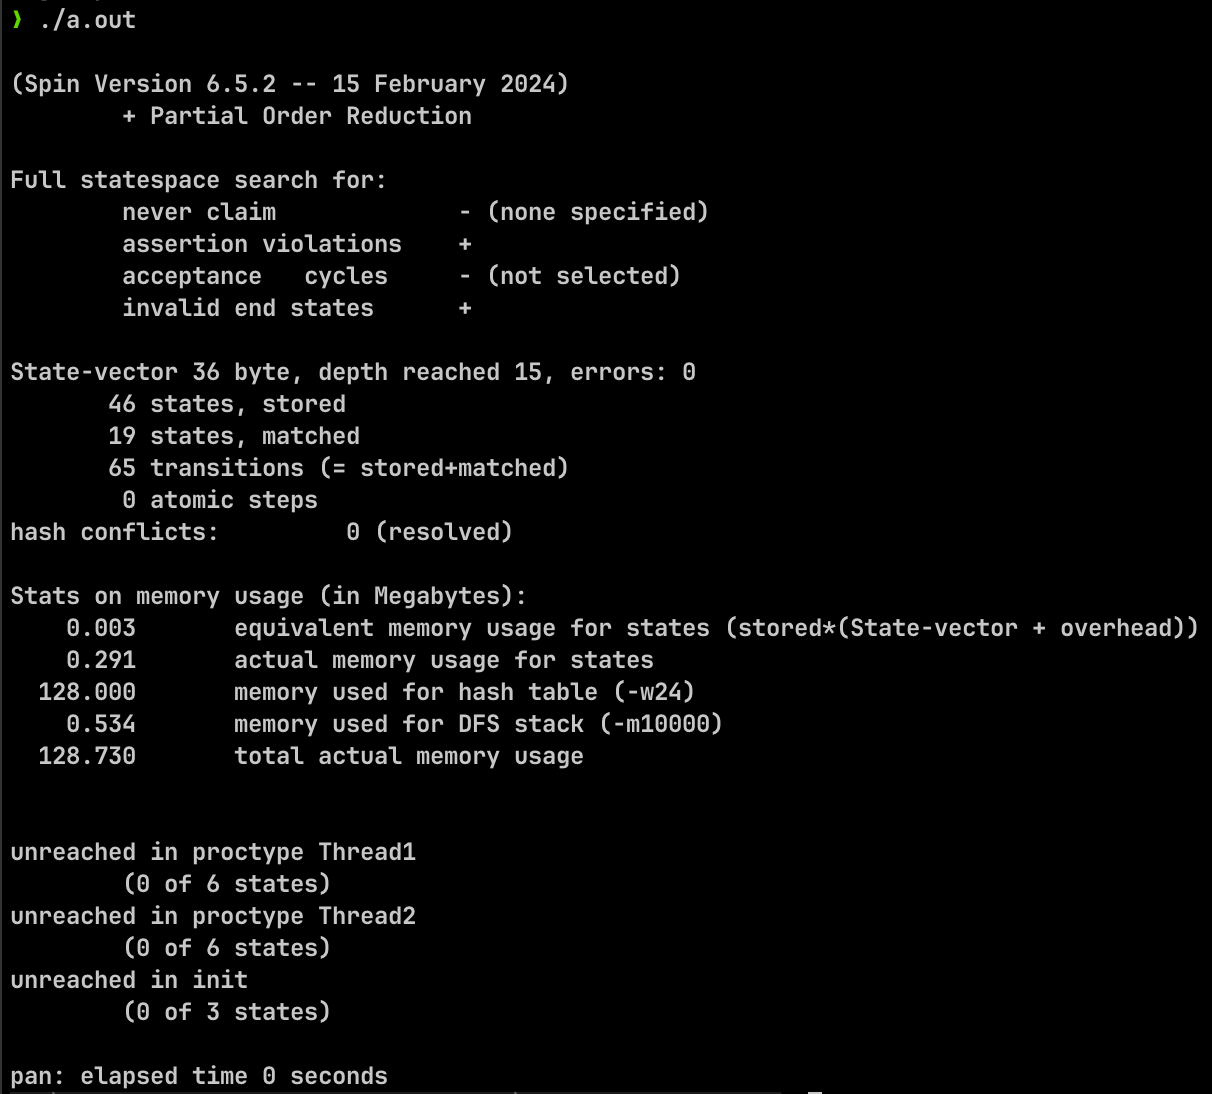
\includegraphics[width=\textwidth]{inc/5.png}
	\caption{ Логи SPIN, демонстрирующие гонку без ассертов. }
	\label{img:5}
\end{figure}

\subsection{Описание модели с мьютексом}

Описание модели представлено в листинге \ref{lst:2}.

\begin{lstlisting}[label=lst:2,caption=Описание модели с мьютексом.]
	short var1 = 3;
	short var2 = 2;
	short res1 = 0;
	
	byte mutex = 0;
	
	proctype Thread1() {
		atomic {
			if
			:: mutex < 1 ->
				mutex++;
				var1++;
				var2++;
				mutex--;
			fi
		}
	}
	
	proctype Thread2() {
		atomic {
			if
			:: mutex < 1 ->
				mutex++;
				res1 = var1 + var2;
				mutex--;
			fi
		}
	}
	
	init {
		atomic {
			run Thread1();
			run Thread2();
		}
	}
\end{lstlisting}

На рисунке \ref{img:4} представлен результат корректного взаимодействия процессов.

\begin{figure}[H]
	\centering
	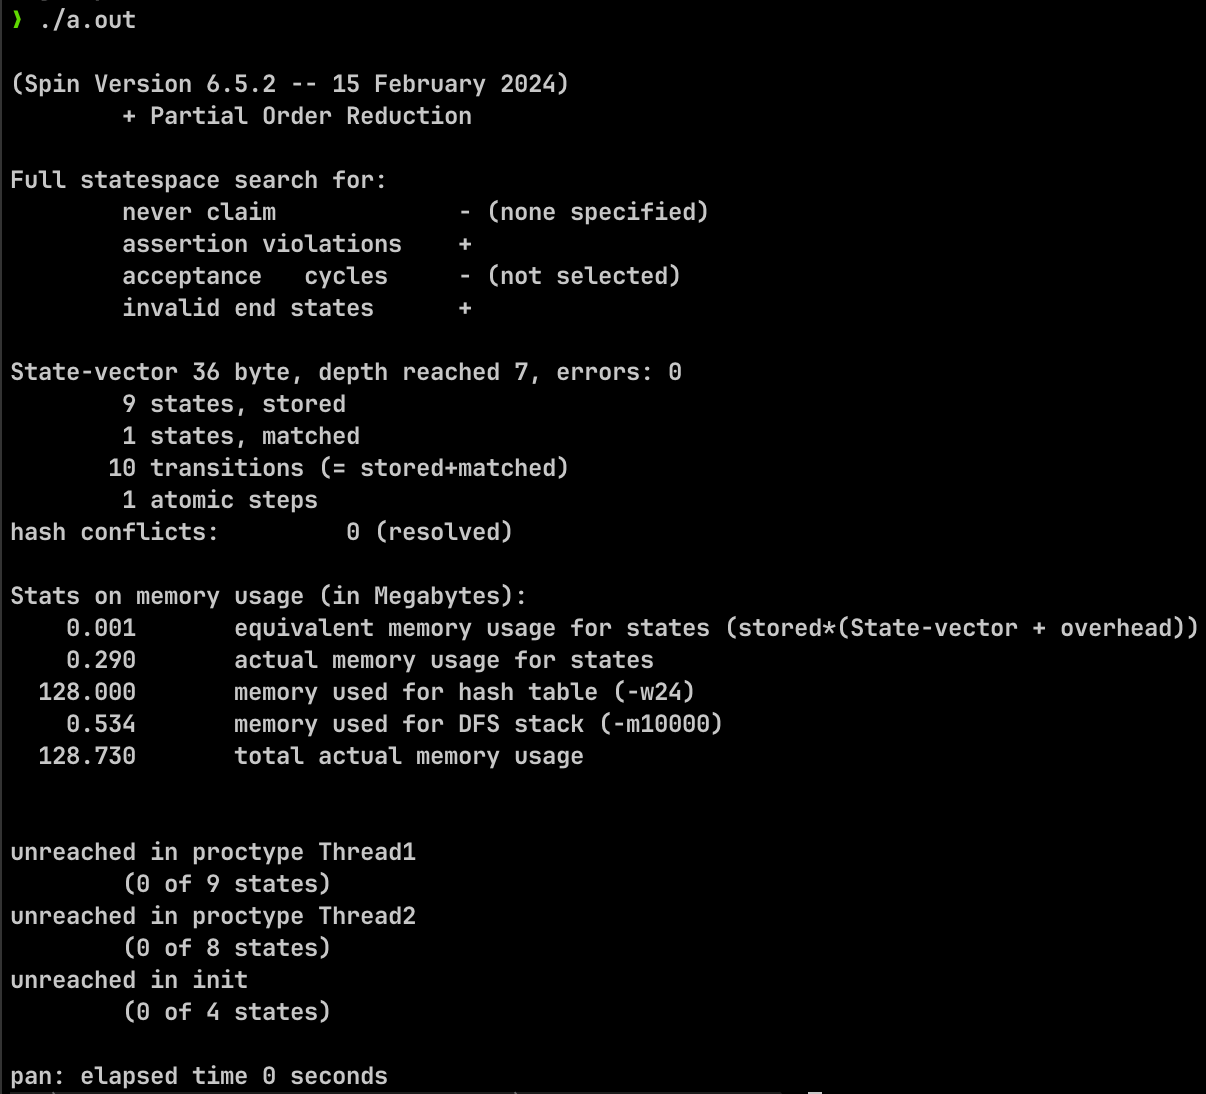
\includegraphics[width=\textwidth]{inc/4.png}
	\caption{ Результат корректного взаимодействия процессов. }
	\label{img:4}
\end{figure}

\pagebreak